\documentclass[10pt,aspectratio=169,serif]{beamer}

\usepackage[fontset=none, scheme=plain]{ctex}
\IfFontExistsTF{Songti SC}{%
	\setCJKmainfont{Songti SC}[AutoFakeSlant=0.2]%
	\setCJKsansfont{Songti SC}[AutoFakeSlant=0.2]%
}{%
	\setCJKmainfont{FandolSong-Regular}[Extension=.otf,BoldFont=FandolSong-Bold,AutoFakeSlant=0.2]%
	\setCJKsansfont{FandolSong-Regular}[Extension=.otf,BoldFont=FandolSong-Bold]%
}
\usepackage{amsmath,amssymb,graphicx,tikz,booktabs,multicol,calligra}
\usepackage{pgfplots}
\pgfplotsset{compat=1.18}
\usepackage{tcolorbox}
\tcbuselibrary{skins}
\usepackage{XyygU}
\usepackage{caption}
\captionsetup[figure]{name=图,labelsep=period}

\usetikzlibrary{arrows.meta,positioning,calc}

\setlength{\abovedisplayskip}{0pt plus 2pt minus 2pt}
\setlength{\belowdisplayskip}{0pt plus 2pt minus 2pt}

\title[习题4.5]{习题 4.5：函数的应用（二）}
\subtitle{复习巩固 \& 综合运用 \& 拓广探索}
\author{}
\institute{}
\date{2026-10-16}

\begin{document}

\begin{frame}
  \titlepage
\end{frame}

% ============================================================
% 第1题：二分法适用条件
% ============================================================
\begin{frame}[t]{第1题：哪些图象不能用二分法求零点}
\textbf{1.} 下列函数图象与 $x$ 轴均有交点，其中不能用二分法求其零点的是 \underline{\quad\quad}（填写所有符合条件的图号）。
\smallskip
\begin{center}
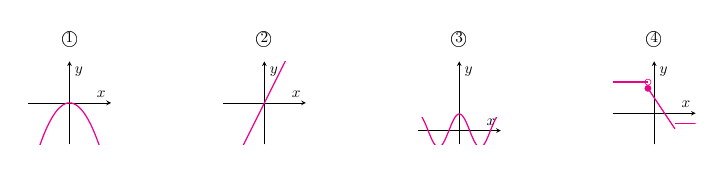
\begin{tikzpicture}[scale=0.55]
% ① 开口向下，顶点在x轴上
\begin{axis}[width=3.5cm,height=3.5cm,axis lines=middle,xtick=\empty,ytick=\empty,
  xlabel={$x$},ylabel={$y$},title={\textcircled{1}},xmin=-2,xmax=2,ymin=-2,ymax=2]
\addplot[thick,magenta,domain=-1.7:1.7,samples=50]{-x^2};
\end{axis}
\begin{scope}[xshift=4.5cm]
\begin{axis}[width=3.5cm,height=3.5cm,axis lines=middle,xtick=\empty,ytick=\empty,
  xlabel={$x$},ylabel={$y$},title={\textcircled{2}},xmin=-2,xmax=2,ymin=-2,ymax=2]
\addplot[thick,magenta,domain=-1.5:1.5,samples=50]{2*x};
\end{axis}
\end{scope}
\begin{scope}[xshift=9cm]
\begin{axis}[width=3.5cm,height=3.5cm,axis lines=middle,xtick=\empty,ytick=\empty,
  xlabel={$x$},ylabel={$y$},title={\textcircled{3}},xmin=-2,xmax=2,ymin=-0.5,ymax=2.5]
\addplot[thick,magenta,domain=-1.8:1.8,samples=100]{0.6*(cos(deg(x*3.14))-1)+0.6};
\end{axis}
\end{scope}
\begin{scope}[xshift=13.5cm]
\begin{axis}[width=3.5cm,height=3.5cm,axis lines=middle,xtick=\empty,ytick=\empty,
  xlabel={$x$},ylabel={$y$},title={\textcircled{4}},xmin=-2,xmax=2,ymin=-1.5,ymax=2.5]
\addplot[thick,magenta,domain=-2:-0.3,samples=2]{1.5};
\addplot[thick,magenta,domain=-0.3:1,samples=50]{1.2-1.5*(x+0.3)};
\addplot[thick,magenta,domain=1:2,samples=2]{-0.5};
\addplot[only marks,mark=o,mark size=2pt,magenta] coordinates {(-0.3,1.5)};
\addplot[only marks,mark=*,mark size=2pt,magenta] coordinates {(-0.3,1.2)};
\end{axis}
\end{scope}
\end{tikzpicture}
\end{center}
\end{frame}

\begin{frame}[t]{第1题 解答}
\begin{tcolorbox}[colback=orange!10,colframe=orange,title=\textbf{解}]
二分法适用条件：① 函数在区间 $[a,b]$ 上\alert{连续}；② $f(a)f(b)<0$（即图象在零点两侧\alert{变号}）。
\smallskip
\begin{itemize}
  \item \textcircled{1}：开口向下的抛物线，顶点与 $x$ 轴相切。零点附近 $f(x)\le 0$，\alert{不变号}，不能用二分法；
  \item \textcircled{2}：直线穿过 $x$ 轴，连续且变号，\alert{可以}用二分法；
  \item \textcircled{3}：曲线始终在 $x$ 轴上方，仅与 $x$ 轴相切，\alert{不变号}，不能用二分法；
  \item \textcircled{4}：在连续下降的斜线段上穿过 $x$ 轴，该段上连续且变号，\alert{可以}用二分法。
\end{itemize}
\smallskip
\textbf{答案：}$\alert{\textcircled{1}\textcircled{3}}$。
\end{tcolorbox}
\end{frame}

% ============================================================
% 第2题：零点存在定理
% ============================================================
\begin{frame}[t]{第2题：由对应值表判断零点区间}
\textbf{2.} 已知函数 $y=f(x)$ 的图象是一条连续不断的曲线，且有如下对应值表：
\smallskip
\begin{center}
\begin{tabular}{c|cccccc}
$x$ & 1 & 2 & 3 & 4 & 5 & 6\\ \hline
$y$ & 136.136 & 15.552 & $-3.92$ & 10.88 & $-52.488$ & $-232.064$
\end{tabular}
\end{center}
函数 $y=f(x)$ 在哪几个区间内一定有零点？为什么？
\end{frame}

\begin{frame}[t]{第2题 解答}
\begin{tcolorbox}[colback=orange!10,colframe=orange,title=\textbf{解}]
由零点存在定理：连续函数若在区间端点处函数值异号，则区间内必有零点。
\smallskip
\begin{itemize}
  \item $f(2)=15.552>0$，$f(3)=-3.92<0$，$f(2)f(3)<0$ $\Rightarrow$ \alert{$(2,3)$ 内有零点}；
  \item $f(3)=-3.92<0$，$f(4)=10.88>0$，$f(3)f(4)<0$ $\Rightarrow$ \alert{$(3,4)$ 内有零点}；
  \item $f(4)=10.88>0$，$f(5)=-52.488<0$，$f(4)f(5)<0$ $\Rightarrow$ \alert{$(4,5)$ 内有零点}。
\end{itemize}
而 $f(1)f(2)>0$、$f(5)f(6)>0$，不能判定。
\smallskip
\textbf{所以 $f(x)$ 一定有零点的区间为：}$\alert{(2,3),\ (3,4),\ (4,5)}$。
\end{tcolorbox}
\end{frame}

% ============================================================
% 第3题：证明方程至少两解
% ============================================================
\begin{frame}[t]{第3题：证明方程至少两个实数解}
\textbf{3.} 已知函数 $f(x)=x^{3}-2x+1$，求证：方程 $f(x)=x$ 在 $(-1,2)$ 内至少有两个实数解。
\end{frame}

\begin{frame}[t]{第3题 解答}
\begin{tcolorbox}[colback=orange!10,colframe=orange,title=\textbf{证明}]
方程 $f(x)=x$ 即
\[
x^{3}-2x+1=x\ \Longleftrightarrow\ g(x)=x^{3}-3x+1=0.
\]
计算端点函数值：
\[
g(0)=1>0,\quad g(1)=1-3+1=-1<0,\quad g(2)=8-6+1=3>0.
\]
\smallskip
\begin{itemize}
  \item $g(0)g(1)<0$，由零点存在定理，方程 $g(x)=0$ 在 $(0,1)$ 内至少有一个实根；
  \item $g(1)g(2)<0$，方程 $g(x)=0$ 在 $(1,2)$ 内至少有一个实根。
\end{itemize}
两个区间不相交，故方程 $f(x)=x$ 在 $(-1,2)$ 内\alert{至少有两个不同的实数解}。
\end{tcolorbox}
\end{frame}

% ============================================================
% 第4题：二分法 ln x - 2/x
% ============================================================
\begin{frame}[t]{第4题：二分法求 $f(x)=\ln x-\dfrac{2}{x}$ 零点}
\textbf{4.} 利用信息技术，用二分法求函数 $f(x)=\ln x-\dfrac{2}{x}$ 的零点（精确度为 $0.1$）。
\end{frame}

\begin{frame}[t]{第4题 解答}
\vspace{-1em}
\begin{tcolorbox}[colback=orange!10,colframe=orange,title=\textbf{解}]
定义域 $x>0$。$f(2)=\ln 2-1\approx -0.307<0$，$f(3)=\ln 3-\tfrac{2}{3}\approx 0.432>0$，零点 $x_{0}\in(2,3)$。
\smallskip
\begin{enumerate}
  \item $c=2.5$，$f(2.5)\approx 0.116>0$ $\Rightarrow x_{0}\in(2,2.5)$；
  \item $c=2.25$，$f(2.25)\approx -0.078<0$ $\Rightarrow x_{0}\in(2.25,2.5)$；
  \item $c=2.375$，$f(2.375)\approx 0.023>0$ $\Rightarrow x_{0}\in(2.25,2.375)$；
  \item $c=2.3125$，$f(2.3125)\approx -0.027<0$ $\Rightarrow x_{0}\in(2.3125,2.375)$。
\end{enumerate}
$|2.375-2.3125|=0.0625<0.1$。
\smallskip
\textbf{零点近似值 } $\alert{x_{0}\approx 2.34}$。
\end{tcolorbox}
\end{frame}

% ============================================================
% 第5题：二分法 0.8^x - 1 = ln x
% ============================================================
\begin{frame}[t]{第5题：二分法求方程 $0.8^{x}-1=\ln x$}
\textbf{5.} 利用信息技术，用二分法求方程 $0.8^{x}-1=\ln x$ 的近似解（精确度为 $0.1$）。
\end{frame}

\begin{frame}[t]{第5题 解答}
\vspace{-1em}
\begin{tcolorbox}[colback=orange!10,colframe=orange,title=\textbf{解}]
令 $f(x)=0.8^{x}-1-\ln x$。$f(0.5)\approx 0.587>0$，$f(1)=-0.2<0$，故 $x_{0}\in(0.5,1)$。
\smallskip
\begin{enumerate}
  \item $c=0.75$，$f(0.75)\approx 0.134>0$ $\Rightarrow x_{0}\in(0.75,1)$；
  \item $c=0.875$，$f(0.875)\approx -0.044<0$ $\Rightarrow x_{0}\in(0.75,0.875)$；
  \item $c=0.8125$，$f(0.8125)\approx 0.042>0$ $\Rightarrow x_{0}\in(0.8125,0.875)$。
\end{enumerate}
$|0.875-0.8125|=0.0625<0.1$。
\smallskip
\textbf{方程近似解为 } $\alert{x\approx 0.84}$。
\end{tcolorbox}
\end{frame}

% ============================================================
% 第6题：计算机病毒
% ============================================================
\begin{frame}[t]{第6题：计算机病毒复制}
\textbf{6.} 一种专门占据内存的计算机病毒，开机时占据内存 $2$ KB，然后每 $3$ 分自身复制一次，复制后所占内存是原来的 $2$ 倍。那么开机后多少分，该病毒会占据 $64$ MB 内存（$1\text{ MB}=1024\text{ KB}$）？
\end{frame}

\begin{frame}[t]{第6题 解答}
\begin{tcolorbox}[colback=orange!10,colframe=orange,title=\textbf{解}]
开机后 $n$ 个 $3$ 分钟周期，病毒占据内存：
\[
y=2\cdot 2^{n}\ \text{KB}.
\]
目标内存：$64\text{ MB}=64\times 1024=65536\text{ KB}$。
\[
2\cdot 2^{n}=65536\ \Rightarrow\ 2^{n}=32768=2^{15}\ \Rightarrow\ n=15.
\]
所需时间：
\[
t=15\times 3=\alert{45\ \text{分钟}}.
\]
\smallskip
\textbf{开机后 }$\alert{45\text{ min}}$\textbf{，病毒占据 }$64\text{ MB}$\textbf{ 内存。}
\end{tcolorbox}
\end{frame}

% ============================================================
% 第7题：证明至少一个零点
% ============================================================
\begin{frame}[t]{第7题：证明二次函数在 $(0,2)$ 内有零点}
\textbf{7.} 设函数 $f(x)=ax^{2}+bx+c\ (a>0,\ b,c\in\mathbf{R})$，且 $f(1)=-\dfrac{a}{2}$，求证：函数 $f(x)$ 在 $(0,2)$ 内至少有一个零点。
\end{frame}

\begin{frame}[t]{第7题 解答}
\begin{tcolorbox}[colback=orange!10,colframe=orange,title=\textbf{证明}]
由 $f(1)=a+b+c=-\dfrac{a}{2}$，得 $b+c=-\dfrac{3a}{2}$。
\smallskip
计算：
\[
f(0)=c,\qquad f(2)=4a+2b+c=a-c.
\]
分情况讨论：
\begin{itemize}
  \item 若 $c(a-c)<0$，即 $f(0)f(2)<0$，则由零点存在定理，$(0,2)$ 内有零点；
  \item 若 $0<c<a$，则 $f(0)=c>0$，$f(2)=a-c>0$，但 $f(1)=-\dfrac{a}{2}<0$，故 $f(0)f(1)<0$ 且 $f(1)f(2)<0$，$(0,1)$ 与 $(1,2)$ 内各有一个零点；
  \item 若 $c=0$，则 $b=-\dfrac{3a}{2}$，$f(x)=ax(x-\tfrac32)$，零点 $x=\tfrac32\in(0,2)$；
  \item 若 $c=a$，则 $b=-\dfrac{5a}{2}$，$f(x)=a(x-\tfrac12)(x-2)$，零点 $x=\tfrac12\in(0,2)$。
\end{itemize}
\textbf{综上，$f(x)$ 在 $(0,2)$ 内至少有一个零点。}
\end{tcolorbox}
\end{frame}

% ============================================================
% 第8题：g(x) = 2 - [f(x)]^2
% ============================================================
\begin{frame}[t]{第8题：复合函数 $g(x)=2-[f(x)]^{2}$}
\textbf{8.} 已知函数 $f(x)=-x^{2}-3x-2$，$g(x)=2-[f(x)]^{2}$。
\begin{enumerate}
  \item 求函数 $y=g(x)$ 的解析式；
  \item 利用信息技术，画出函数 $y=g(x)$ 的图象；
  \item 求函数 $y=g(x)$ 的零点（精确度为 $0.1$）。
\end{enumerate}
\end{frame}

\begin{frame}[t]{第8题 解答}
\begin{tcolorbox}[colback=orange!10,colframe=orange,title=\textbf{解}]
\textbf{(1)} $f(x)=-(x+1)(x+2)$，故
\[
g(x)=2-(x+1)^{2}(x+2)^{2}.
\]
\smallskip
\textbf{(3)} 令 $g(x)=0$：
\[
(x+1)^{2}(x+2)^{2}=2\ \Rightarrow\ (x+1)(x+2)=\pm\sqrt{2}.
\]
\begin{itemize}
  \item $(x+1)(x+2)=\sqrt{2}$：$x^{2}+3x+2-\sqrt{2}=0$，$\Delta=9-4(2-\sqrt{2})=1+4\sqrt{2}>0$，两根 $x\approx -0.42,\ -2.58$；
  \item $(x+1)(x+2)=-\sqrt{2}$：$x^{2}+3x+2+\sqrt{2}=0$，$\Delta=9-4(2+\sqrt{2})<0$，无实根。
\end{itemize}
\textbf{零点为 } $\alert{x_{1}\approx -2.58,\quad x_{2}\approx -0.42}$。
\end{tcolorbox}
\end{frame}

% ============================================================
% 第9题：浮萍 y = a^t
% ============================================================
\begin{frame}[t]{第9题：浮萍面积模型}
\textbf{9.} 如图，某池塘里浮萍的面积 $y$（单位：$\text{m}^{2}$）与时间 $t$（单位：月）的关系为 $y=a^{t}$。关于下列说法：
\begin{center}
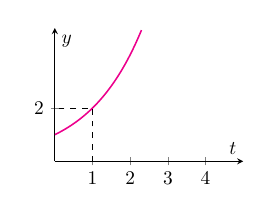
\begin{tikzpicture}[scale=0.7]
\begin{axis}[width=5cm,height=4cm,axis lines=middle,xtick={1,2,3,4},ytick={2},
  xlabel=$t$,ylabel=$y$,xmin=0,xmax=5,ymin=0,ymax=5]
\addplot[thick,magenta,domain=0:2.3,samples=50]{2^x};
\draw[dashed] (axis cs:1,0) -- (axis cs:1,2) -- (axis cs:0,2);
\end{axis}
\end{tikzpicture}
\end{center}
\begin{enumerate}
  \item 浮萍每月的增长率为 $1$；
  \item 第 $5$ 个月时，浮萍面积就会超过 $30\text{ m}^{2}$；
  \item 浮萍每月增加的面积都相等；
  \item 若浮萍蔓延到 $2\text{ m}^{2},3\text{ m}^{2},6\text{ m}^{2}$ 所经过时间分别为 $t_{1},t_{2},t_{3}$，则 $t_{1}+t_{2}=t_{3}$。
\end{enumerate}
其中正确的说法是（\quad）。\\
(A) \textcircled{1}\textcircled{2}\quad (B) \textcircled{1}\textcircled{2}\textcircled{3}\quad (C) \textcircled{1}\textcircled{2}\textcircled{4}\quad (D) \textcircled{1}\textcircled{2}\textcircled{3}\textcircled{4}
\end{frame}

\begin{frame}[t]{第9题 解答}
\begin{tcolorbox}[colback=orange!10,colframe=orange,title=\textbf{解}]
由图知 $t=1$ 时 $y=2$，故 $a=2$，即 $y=2^{t}$。
\smallskip
\begin{itemize}
  \item \textcircled{1} 月增长率 $=\dfrac{2^{t+1}-2^{t}}{2^{t}}=1=100\%$，\textbf{正确}；
  \item \textcircled{2} $t=5$ 时 $y=2^{5}=32>30$，\textbf{正确}；
  \item \textcircled{3} 月增加量 $2^{t+1}-2^{t}=2^{t}$ 随 $t$ 增大而增大，\textbf{错误}；
  \item \textcircled{4} $2^{t_{1}}=2\Rightarrow t_{1}=1$；$2^{t_{2}}=3\Rightarrow t_{2}=\log_{2}3$；$2^{t_{3}}=6\Rightarrow t_{3}=\log_{2}6$。
  $t_{1}+t_{2}=1+\log_{2}3=\log_{2}2+\log_{2}3=\log_{2}6=t_{3}$，\textbf{正确}。
\end{itemize}
\textbf{答案：}$\alert{\text{(C) \textcircled{1}\textcircled{2}\textcircled{4}}}$。
\end{tcolorbox}
\end{frame}

% ============================================================
% 第10题：药物衰减
% ============================================================
\begin{frame}[t]{第10题：血液中药量衰减}
\textbf{10.} 一种药在病人血液中的量保持在 $1500$ mg 以上时才有疗效，而低于 $500$ mg 时病人就有危险。现给某病人静脉注射了这种药 $2500$ mg，如果药在血液中以每小时 $20\%$ 的比例衰减，那么应在什么时间范围再向病人血液补充这种药（精确到 $0.1$ h）？
\end{frame}

\begin{frame}[t]{第10题 解答}
\begin{tcolorbox}[colback=orange!10,colframe=orange,title=\textbf{解}]
注射后 $t$ 小时，血中药量：
\[
y=2500\cdot 0.8^{t}\ \text{mg}.
\]
\textbf{有效下限（药量降到 $1500$ mg）：}
\[
2500\cdot 0.8^{t}=1500\Rightarrow 0.8^{t}=0.6
\Rightarrow t=\frac{\ln 0.6}{\ln 0.8}\approx 2.3\ \text{h}.
\]
\textbf{危险下限（药量降到 $500$ mg）：}
\[
2500\cdot 0.8^{t}=500\Rightarrow 0.8^{t}=0.2
\Rightarrow t=\frac{\ln 0.2}{\ln 0.8}\approx 7.2\ \text{h}.
\]
\smallskip
\textbf{应在注射后 } $\alert{2.3\text{ h} \sim 7.2\text{ h}}$ \textbf{之间再次补充药物}（不能晚于 $7.2$ h，否则有危险）。
\end{tcolorbox}
\end{frame}

% ============================================================
% 第11题：全球数据量
% ============================================================
\begin{frame}[t]{第11题：全球数据量增长模型}
\textbf{11.} 2008 年全球产生的数据量为 $0.49$ ZB，2009 年为 $0.8$ ZB，2010 年为 $1.2$ ZB，2011 年为 $1.82$ ZB。
\begin{enumerate}
  \item 从 $f(x)=kx+b$ 和 $g(x)=ab^{x}$ 中选择一个，求出解析式；
  \item 估计 2018 年全球数据量，并与公布数据比较。
\end{enumerate}
\end{frame}

\begin{frame}[t]{第11题 解答}
\begin{tcolorbox}[colback=orange!10,colframe=orange,title=\textbf{解}]
设 $x$ 为距 2008 年的年数。数据增量 $0.31,0.4,0.62$ 逐渐增大，呈加速增长，故选\alert{指数模型} $g(x)=ab^{x}$。
\smallskip
用 $(0,0.49)$、$(3,1.82)$：$a=0.49$，$b^{3}=\dfrac{1.82}{0.49}\approx 3.714$，$b\approx 1.55$。
\[
g(x)=0.49\times 1.55^{x}.
\]
验证：$g(1)\approx 0.76$（实际 $0.8$），$g(2)\approx 1.17$（实际 $1.2$），吻合良好。
\smallskip
\textbf{(2)} 2018 年对应 $x=10$：
\[
g(10)=0.49\times 1.55^{10}\approx 0.49\times 80\approx \alert{39\ \text{ZB}}.
\]
（实际 2018 年全球数据量已超 $40$ ZB，模型估计基本合理，但指数增长在后期可能进一步加速。）
\end{tcolorbox}
\end{frame}

% ============================================================
% 第12题：身高体重
% ============================================================
\begin{frame}[t]{第12题：身高与体重模型}
\textbf{12.} 某地不同身高未成年男性平均体重如下：
\smallskip
\begin{center}
\begin{tabular}{l|ccccccccccc}
身高/cm & 60&70&80&90&100&110&120&130&140&150&160&170\\ \hline
体重/kg & 6.13&7.90&9.99&12.15&15.02&17.50&20.92&26.86&31.11&38.85&47.25&55.05
\end{tabular}
\end{center}
\begin{enumerate}
  \item 建立函数模型反映平均体重 $y$ 与身高 $x$ 的关系；
  \item 体重超过同身高男性平均值 $1.2$ 倍为偏胖，低于 $0.8$ 倍为偏瘦。身高 $175$ cm、体重 $78$ kg 的男生是否正常？
\end{enumerate}
\end{frame}

\begin{frame}[t]{第12题 解答}
\begin{tcolorbox}[colback=orange!10,colframe=orange,title=\textbf{解}]
\textbf{(1)} 体重近似与身高平方成正比（体积 $\propto$ 身高$^{3}$，但未成年期介于 $x^{2}$ 与 $x^{3}$ 之间，取二次模型）。用端点 $(60,6.13)$、$(170,55.05)$：
\[
y\approx 0.0019\,x^{2}.
\]
（验证 $x=100$：$19.0$ kg，实际 $15.0$ kg；模型为近似，趋势吻合。）
\smallskip
\textbf{(2)} $x=175$ 时：
\[
y\approx 0.0019\times 175^{2}\approx 58.2\ \text{kg}.
\]
上限：$1.2\times 58.2\approx 69.8$ kg。实际体重 $78>69.8$。
\smallskip
\textbf{该男生 }$\alert{\text{偏胖}}$。
\end{tcolorbox}
\end{frame}

% ============================================================
% 第13题：恰有一个零点
% ============================================================
\begin{frame}[t]{第13题：辨析"恰有一个零点"}
\textbf{13.} 一道题："若函数 $f(x)=24ax^{2}+4x-1$ 在区间 $(-1,1)$ 内恰有一个零点，求实数 $a$ 的取值范围"。某同学解答：
\[
f(-1)f(1)=(24a-5)(24a+3)<0\ \Rightarrow\ -\frac{1}{8}<a<\frac{5}{24}.
\]
上述解答正确吗？若不正确，说明理由并给出正确解答。
\end{frame}

\begin{frame}[t]{第13题 解答}
\begin{tcolorbox}[colback=orange!10,colframe=orange,title=\textbf{解：不正确}]
该同学只考虑了 $f(-1)f(1)<0$ 的情形，遗漏了以下情况：
\smallskip
\begin{itemize}
  \item \textbf{$a=0$：} $f(x)=4x-1$，零点 $x=\tfrac14\in(-1,1)$，应包含；
  \item \textbf{重根在区间内：} $\Delta=16+96a=0\Rightarrow a=-\tfrac16$。此时 $f(x)=-(2x-1)^{2}$，二重根 $x=\tfrac12\in(-1,1)$，恰一个零点，应包含；
  \item \textbf{端点零点：} $f(-1)=0\Rightarrow a=\tfrac{5}{24}$，另一根 $x=\tfrac15\in(-1,1)$；$f(1)=0\Rightarrow a=-\tfrac18$，另一根 $x=\tfrac13\in(-1,1)$。端点值应闭区间包含。
\end{itemize}
\smallskip
\textbf{正确答案：}
\[
\alert{a=-\frac{1}{6},\quad \text{或}\quad -\frac{1}{8}\le a\le \frac{5}{24}}.
\]
\end{tcolorbox}
\end{frame}

% ============================================================
% 第14题：汽车耗油量
% ============================================================
\begin{frame}[t]{第14题：汽车耗油量与速度}
\textbf{14.} 甲地到乙地 $240$ km。实验得汽车每小时耗油量 $Q$（L）与速度 $v$（km/h）$(0\le v\le 120)$：
\smallskip
\begin{center}
\begin{tabular}{c|ccccc}
$v$ & 0 & 40 & 60 & 80 & 120\\ \hline
$Q$ & 0.000 & 6.667 & 8.125 & 10.000 & 20.000
\end{tabular}
\end{center}
备选模型：$Q=av^{3}+bv^{2}+cv$，$Q=0.5^{v}+a$，$Q=k\log_{a}v+b$。
\begin{enumerate}
  \item 选最符合实际的模型并求解析式；
  \item 该车应以何速度行驶总耗油最少？
\end{enumerate}
\end{frame}

\begin{frame}[t]{第14题 解答}
\begin{tcolorbox}[colback=orange!10,colframe=orange,title=\textbf{解}]
\textbf{(1)} $v=0$ 时 $Q=0$，排除对数模型（$v=0$ 无定义）和指数模型（$v=0$ 时 $Q=1+a\ne 0$）。故选三次模型：
\[
Q=av^{3}+bv^{2}+cv.
\]
用 $(40,6.667),(60,8.125),(80,10)$ 解得：
\[
a\approx 2.6\times 10^{-5},\quad b\approx -4.2\times 10^{-3},\quad c\approx 0.29.
\]
验证 $v=120$：$Q\approx 20.0$，吻合。
\smallskip
\textbf{(2)} 总耗油量 $=Q\cdot\dfrac{240}{v}=240\cdot\dfrac{Q}{v}$，最小化 $\dfrac{Q}{v}=av^{2}+bv+c$。
顶点：
\[
v=-\frac{b}{2a}=\frac{4.2\times 10^{-3}}{2\times 2.6\times 10^{-5}}\approx \alert{80\ \text{km/h}}.
\]
\textbf{以 }$\alert{80\text{ km/h}}$\textbf{ 匀速行驶总耗油最少。}
\end{tcolorbox}
\end{frame}

\begin{frame}[c]
  \begin{center}
    {\Huge\calligra Thanks!}
  \end{center}
\end{frame}

\end{document}
